\documentclass[12pt]{spieman}  % 12pt font required by SPIE;
%\documentclass[a4paper,12pt]{spieman}  % use this instead for A4 paper
\usepackage{amsmath,amsfonts,amssymb}
\usepackage{graphicx}
\usepackage{setspace}
\usepackage{tocloft}
\usepackage{lscape}

\usepackage{float} % Added to keep pictures where they belong
% Reference for this fix: https://tex.stackexchange.com/questions/8625/force-figure-placement-in-text

\usepackage{listings}
\usepackage{color}
\usepackage{textcomp}
\definecolor{listinggray}{gray}{0.9}
\definecolor{lbcolor}{rgb}{0.9,0.9,0.9}
\lstset{
	numbers=left,
    xleftmargin=2em,
    xrightmargin=1em,
	tabsize=4,
	rulecolor=,
	language=Bash,
        basicstyle=\scriptsize,
        upquote=true,
        aboveskip={1.5\baselineskip},
        columns=fixed,
        showstringspaces=false,
        extendedchars=true,
        breaklines=true,
        prebreak = \raisebox{0ex}[0ex][0ex]{\ensuremath{\hookleftarrow}},
        frame=0L,
        showtabs=false,
        showspaces=false,
        showstringspaces=false,
        identifierstyle=\ttfamily,
        keywordstyle=\color[rgb]{0,0,1},
        commentstyle=\color[rgb]{0.133,0.545,0.133},
        stringstyle=\color[rgb]{0.627,0.126,0.941},
		rulecolor=\color{black},
}

\title{A Comparison of Pre-Built Hypervisors}

\author[a]{Taylor Chien}
\affil[a]{SUNY Polytechnic Institute, Computer Science Department, 100 Horatio Street, Utica, NY, 13502}

\renewcommand{\cftdotsep}{\cftnodots}
\cftpagenumbersoff{figure}
\cftpagenumbersoff{table} 
\begin{document} 
\maketitle

\begin{abstract}
There are a lot of Hypervisors out there, from almost every developer. VMWare isn't the only option anymore, with free and open-source hypervisors everywhere now. However, in terms of usability, building a system from scratch is something that only advanced users should attempt.\\

I decided that I should compare the most popular hypervisors to each other and see if there was actually any differences in performance. The original list ranged from open-source-based options to Microsoft, VMWare, and Solaris, but eventually, I settled on four that were easily accessible, widely used, and free (ESXi has a 60 day trial).

\end{abstract}

%\begin{spacing}{2}   % use double spacing for rest of manuscript

\section{Introduction}

Hypervisors are the systems that manage how a virtualization cluster operates. There are several well-known software options, including software like Oracle’s Virtualbox, VMware’s vPlayer, and Microsoft’s Hyper-V, along with open-source solutions such as oVirt and OpenStack.\\

These solutions usually run on top of another operating system, such as Windows or Linux. Instead of doing that, these pre-built hypervisors are built so that they do not need another program to run, and can be installed straight to hardware, turning an entire server into a virtual host.\\

What these special operating systems do is take the software and integrate it with tools that manage the operating systems and what runs on it. This usually allows for functions such as pooling and clustering, where multiple servers are joined together and work as one unit. With a pre-built solution there is also no risk of a compatibility bug or improperly configured package disabling the entire installation.\\

Most modern operating systems, including all Windows platforms and some specialized Linux operating systems, virtualize or containerize their programs to isolate them from other operating system components. This allows Windows platforms to launch a previous version of the kernel for backwards compatibility, or simply separate a potentially vulnerable program from the rest of  the computer’s files in a process known as “sandboxing”.\\

Virtualization is a very important technology in the modern datacenter, allowing thousands of systems to be run on comparatively little hardware, or for Virtual Provisioning Services such as Amazon Web Services or Digitalocean to sell space on their clusters for businesses or enthusiasts to buy.\\

Currently, there are four main competing pre-built packages. These are:
\begin{itemize}
\item Proxmox VE
\item Citrix XenServer
\item Hyper-V Server
\item VMWare vSphere/ESXi
\end{itemize}

\section{Literature Review}

Each of the hypervisors has a small blurb about themselves on their website. They all are meant to do the same thing, but their focus group is different.

Proxmox has information on their site primarily focused on their open source project and the system's features. Their website states that the software is Enterprise focused with "an intuitive interface"\cite{proxmoxweb}. They boast Linux and Windows compatibility along with high availability and containerization.

XenServer, which is owned by Citrix, also states that it is an enterprise-class solution. However, unlike Proxmox, XenServer focuses heavily on their management and scalability features. These features include power management for servers, multiple server management from a single interface, and performance alerts\cite{xenserverweb}.

Hyper-V does not state anything about its enterprise use. Instead, they focus on efficiency and capacity expansion, and its use as a personal cloud\cite{hypervweb}. Most of the information page is focused on its use for expanding the capabilities of Windows Server operating systems, allowing Linux machines to be run in parallel.

VMware's ESXi page is focused on their capabilities and how it can help consolidate an environment. It also fails to mention that the ESXi's "Free Download" is a 60-day  trial.\cite{vmwareweb}

\section{Methods and Materials}
\label{sec:met-mat}

The testing and analysis procedures will be broken into four main stages, which will each focus on a different set of tasks. This will allow for easy replication of the work done here, along with the ability to note as many differences as possible between the four hypervisors.\\

The devices used for this test will be fourteen Dell 860 servers, each with 4 GB of RAM, a dual-core Xeon 3050 CPU, and two 80 GB hard drives. These CPUs have virtualization extensions and demand-based power management enabled.

\subsection{Eliminating Variables}
\label{subsec:variables}

In order to eliminate any level of difference in the actual hardware, several measures will be taken to balance out any issues. The primary issue with this is that some of the hard drives may be from different generations, and these servers to not have hardware RAID cards to balance the two disks.  Two steps will be taken to eliminate this.\\

First, during the bare metal testing of the chosen guest operating systems, two servers with identical drives will be chosen, and then those drives will be placed in RAID 1 to balance any disk issues.\\

While this will work for the guest operating systems, not all of the hypervisors can use this method to even out potential slower disks. While Proxmox can use ZFS RAID 1, none of the other hypervisors can. Instead what will happen is that when the guest VMs are built, their hard drives will be placed on an iSCSI share on a central server, equalizing their disk speeds. This may cause an overall slowdown, but any differences between the guests should then only be because of the hypervisor and not the disks.

\subsection{Initial Setup}
\label{subsec:initial-setup}

The initial setup will consist of twelve servers dedicated to testing the Hypervisor hosts and their guests. Initially, two of the servers will be used to centralize several services on the network.\\

The first server, "Enterprise" will be used as the central iSCSI and storage server. This server will be using two 750 GB Hard Drives in RAID 1, and then splitting those drives into seven 100GB sections using LVM. Four of the 100 GB sections will be used for iSCSI, with one target and LUN for each virtualization host. The fifth 100 GB section will be used for testing backups. The sixth and seventh 100 GB sections will be used as an NFS and Samba share respectively for ISO images of the guest operating systems.\\

The second server, "Yorktown", will be the central point for documentation when the project is complete, with two 750 GB Hard Drives in RAID 1, but no division of the disk. Instead it will be running the web service ownCloud, where documentation can be placed once the project is complete.\\

Also set up are a Windows 10 desktop, for installing XenServer and VMwares` Windows-only clients, and a Ubuntu Desktop client, for easy server management through SSH.

\subsection{Stage 1: Hardware Benchmarks}
\label{subsec:stage-1}

Before I even start my hypervisor test though, I need to benchmark the operating systems that I will be using as guests later on. Debian and CentOS cover a large user base, although the reason I'm using them is that Proxmox is based off of Debian, and XenServer is based off CentOS, which allows para-virtualization to come into play on these two systems, potentially boosting speeds.\\

These operating systems will be the absolute bare minimum with no extra packages, services, or other configuration, so that when the time comes to install them on a hypervisor, the process will be identical.\\

The only difference will be that on the hardware, they will have two hard drives placed in software RAID. When they are virtualized, that RAID array will be on the iSCSI server that they are accessing.\\

The tests that will be run are:

\begin{itemize}
\item iPerf two-way Network Speed Test run on the LAN
\item Sysbench (CPU, Disk, RAM [with small, medium, and large filesizes])
\item OpenSSL Speed Test (watching only md5, sha1, aes-256 cbc, sha512, rsa 4096 sign/s and verify/s)
\end{itemize}

This process will be repeated three times with a one minute delay between the runs. This will be the baseline that all of the other guests will be compared to.

\subsection{Stage 2: Hypervisor Installation}
\label{subsec:stage-2}
In order to provide a complete comparison, I'll be documenting the installation of each of these hypervisors and any oddities in their process. For example, if USB installation does not work for Proxmox, or if vSphere spins up a VM in order to configure the cluster instead of using the host, that will be documented.\\

This stage is for documenting exactly what I did to install the system and showing how different they really are from one another.\\

This will also help show how accessing each cluster will be different from each other. Proxmox uses a web GUI while XenServer uses a Windows client or XAPI system from Xen. With these differences come accessibility issues on some platforms.\\

Finally, this will show how installing the operating systems will be different for each. Both Xenserver and Proxmox may paravirtualize their compatible host OSes, making them much faster, but Hyper-V may not even be able to run VMs due to very high hardware requirements. Again, the default options will be chosen for each.

\subsection{Stage 3: Guest Benchmarks}
\label{subsec:stage-3}

Each hypervisor will be given two guests, each with 1 GB of RAM, a 10 GB storage disk, and a single CPU core. Once these are installed with the same configuration (Debian installed without LVM, CentOS using default automatic partitioning) they will be updated and the same tests as above will be run.

\subsection{Benchmarking Script}
\label{subsec:script}

To automate the process, I wrote a script that performed all of these tests in sequence so that the results could be reliable.

\lstinputlisting{Scripts/sysbench.sh}

This generates a single file for the entire benchmark, which makes entering the details into a spreadsheet much easier.

\subsubsection{Testing Rational}
\label{subsec:rational}

Each test was run to test the speed of a certain part of the system, from memory speed to network capacity. Some tests were verification of certain aspects of the system's operation.

The iPerf tests were as much of a test of network throughput as the network's capacity. Reduced numbers could indicate a problem or some kind of overhead with the virtual switch.

\section{Results}

Measured results are numerical values derived from the benchmarking tests. 
% The results for this test will be broken up into two sections: Measured and Observed. Observed results are those that cannot be categorically measured, such as processes for installation.\\

Hyper-V's results for the measured section are not shown because Hyper-V Server would not run VMs due to a non-compatible CPU. This issue was caused by the Core 2 Duo based Xeon 3050 not having SLAT (Second Level Address Translation) support. This is only an issue for Hyper-V.

\subsection{Measured}

The measured results will be split into three sections based on the type of benchmark that was run. Some results were omitted due to all measurements ending up the same, including the Total Time for the Sysbench Disk test (300), and the Average Time for the Sysbench 1KB RAM Test (0).

\subsubsection{OpenSSL Speed}

\begin{figure}[H]
\caption{MD5 OpenSSL - Higher is Better}
\centering
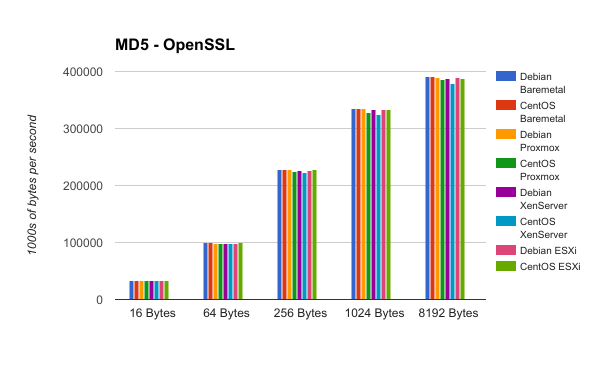
\includegraphics[width=\textwidth,keepaspectratio]{Graphs/MD5-OpenSSL}
\end{figure}

\begin{figure}[H]
\caption{SHA1 OpenSSL - Higher is Better}
\centering
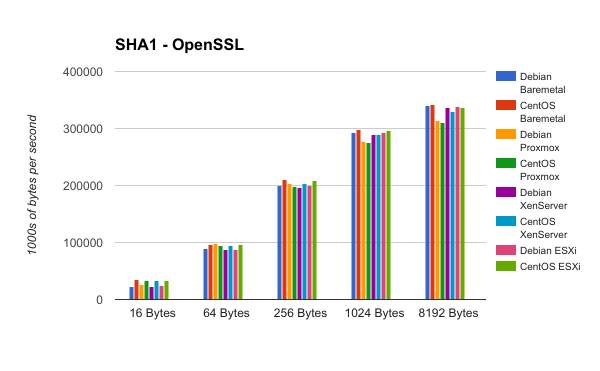
\includegraphics[width=\textwidth,keepaspectratio]{Graphs/SHA1-OpenSSL}
\end{figure}

\begin{figure}[H]
\caption{AES256 OpenSSL - Higher is Better}
\centering
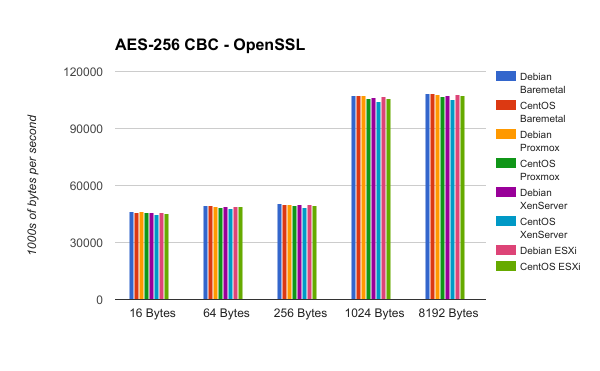
\includegraphics[width=\textwidth,keepaspectratio]{Graphs/AES256-OpenSSL}
\end{figure}

\begin{figure}[H]
\caption{SHA512 OpenSSL - Higher is Better}
\centering
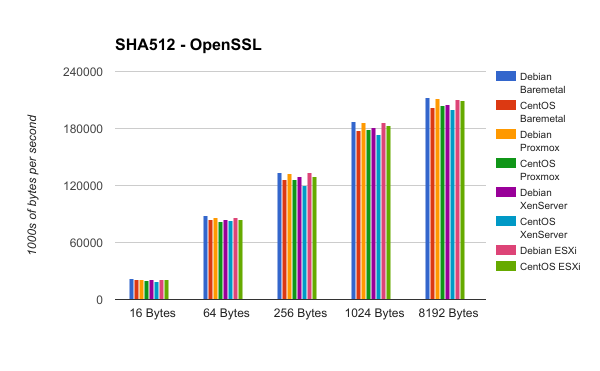
\includegraphics[width=\textwidth,keepaspectratio]{Graphs/SHA512-OpenSSL}
\end{figure}

\begin{figure}[H]
\caption{RSA Sign/s OpenSSL - Higher is Better}
\centering
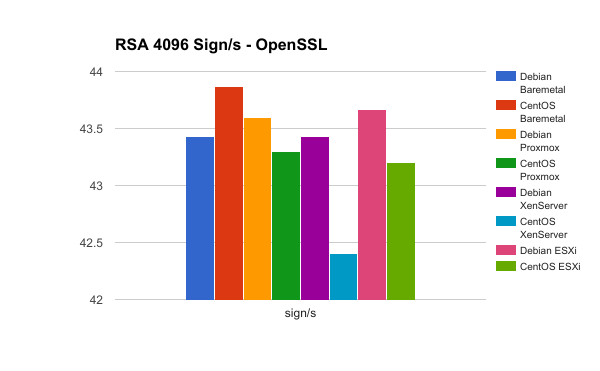
\includegraphics[width=\textwidth,keepaspectratio]{Graphs/RSA-Sign-OpenSSL}
\end{figure}

\begin{figure}[H]
\caption{RSA Verify/s OpenSSL - Higher is Better}
\centering
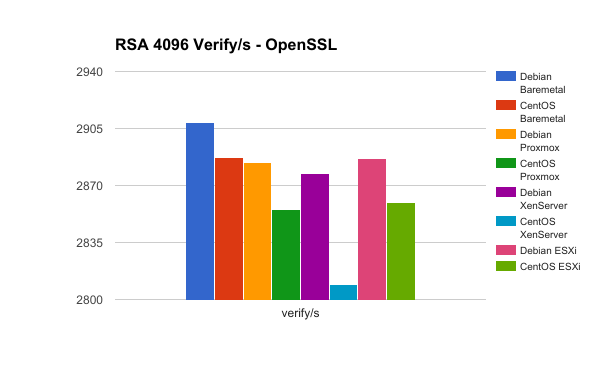
\includegraphics[width=\textwidth,keepaspectratio]{Graphs/RSA-Verify-OpenSSL}
\end{figure}

\subsubsection{iPerf}

\begin{figure}[H]
\caption{Bandwidth - iPerf - Higher is Better}
\centering
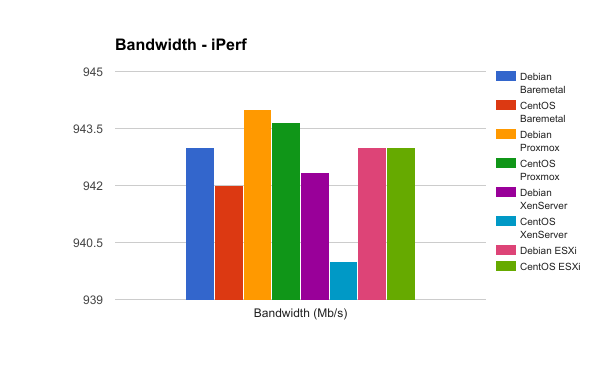
\includegraphics[width=\textwidth,keepaspectratio]{Graphs/Bandwidth-iPerf}
\end{figure}

\subsubsection{Sysbench}

The sysbench test suite is used to benchmark systems in multiple ways. The tests run here were on the CPU, Hard Drive, and RAM.\\

\begin{figure}[H]
\caption{Disk Average - Sysbench - Lower is Better}
\centering
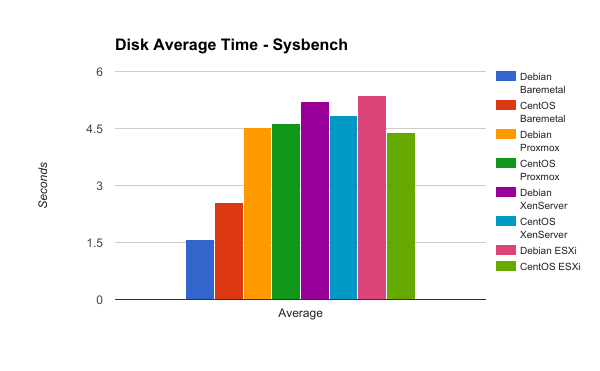
\includegraphics[width=\textwidth,keepaspectratio]{Graphs/Disk-Average-Sysbench}
\end{figure}

\begin{figure}[H]
\caption{CPU Total Time - Sysbench - Lower is Better}
\centering
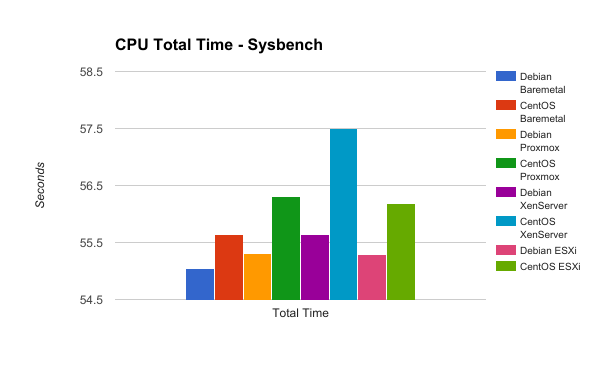
\includegraphics[width=\textwidth,keepaspectratio]{Graphs/CPU-Total-Sysbench}
\end{figure}

\begin{figure}[H]
\caption{CPU Average Time - Sysbench - Lower is Better}
\centering
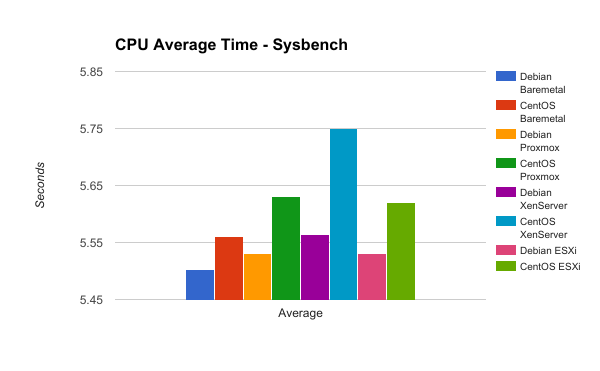
\includegraphics[width=\textwidth,keepaspectratio]{Graphs/CPU-Average-Sysbench}
\end{figure}

\begin{figure}[H]
\caption{RAM 1K Transfer Total Time - Sysbench - Lower is Better}
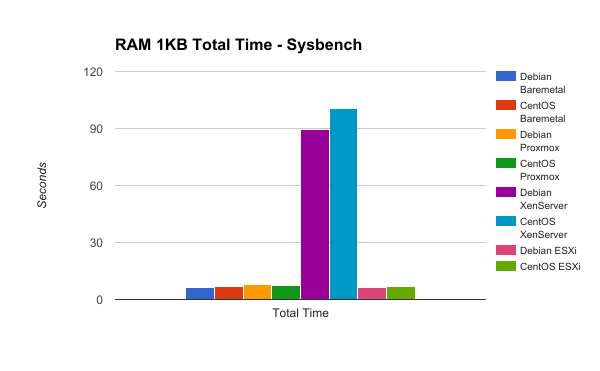
\includegraphics[width=\textwidth,keepaspectratio]{Graphs/RAM-1K-Total}
\end{figure}

\begin{figure}[H]
\caption{RAM 1M Transfer Total Time - Sysbench - Lower is Better}
\centering
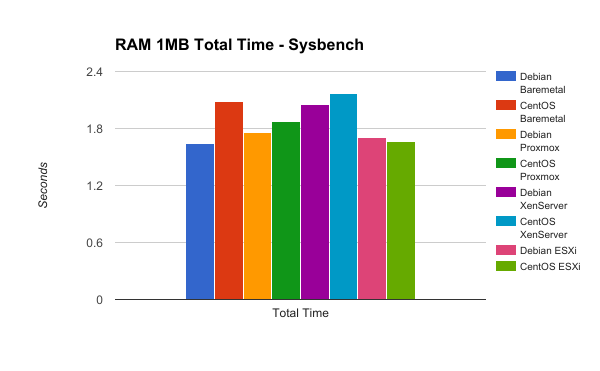
\includegraphics[width=\textwidth,keepaspectratio]{Graphs/RAM-1M-Total}
\end{figure}

\begin{figure}[H]
\caption{RAM 1M Transfer Average Time - Sysbench - Lower is Better}
\centering
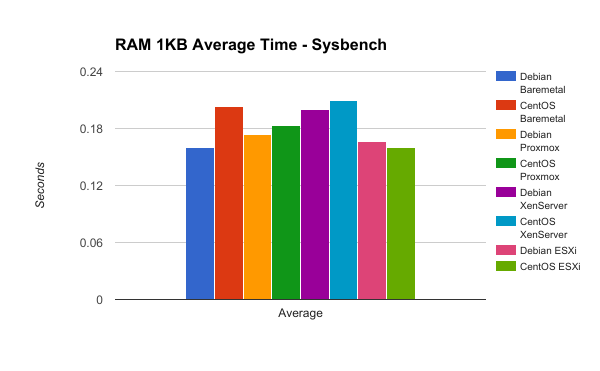
\includegraphics[width=\textwidth,keepaspectratio]{Graphs/RAM-1M-Average}
\end{figure}

\begin{figure}[H]
\caption{RAM 1G Transfer Total Time - Sysbench - Lower is Better}
\centering
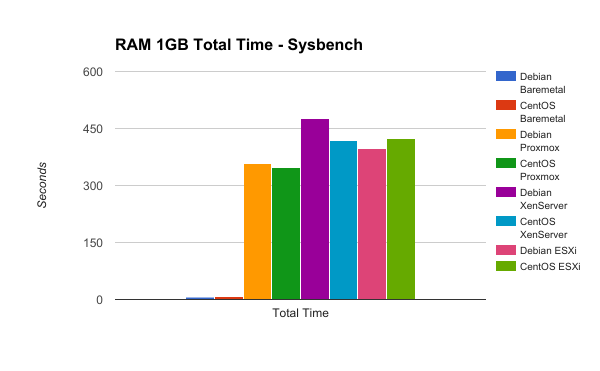
\includegraphics[width=\textwidth,keepaspectratio]{Graphs/RAM-1G-Total}
\end{figure}

\begin{figure}[H]
\caption{RAM 1G Transfer Average Time - Sysbench - Lower is Better}
\centering
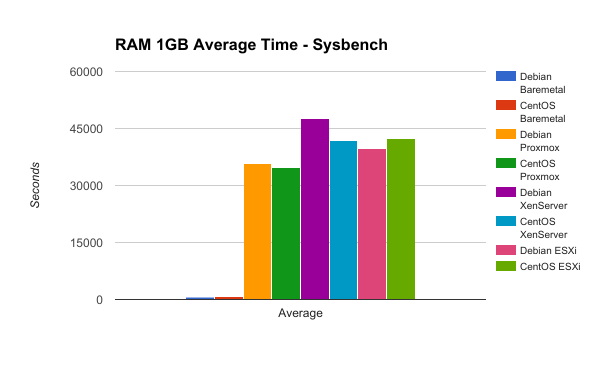
\includegraphics[width=\textwidth,keepaspectratio]{Graphs/RAM-1G-Average}
\end{figure}

\subsection{Errors}

\subsubsection{Proxmox ISO Imaging}

When installing Proxmox over USB devices such as Flash Drives or External CD Drives, proper procedures must be followed. Proxmox will not recognize USB devices such as external CD or USB drives as usable installation media, unless that device is a USB drive formatted in a certain way. This can cause major problems when using ISO writers, since what Proxmox actually wants is a clone of the ISO file on the disk, not the ISO partitions. USB CD drives will not work at all, since when Proxmox is searching for its CD drive it will not find it since certain modules aren't available.

\subsubsection{RAID Partitions on Hard Drives break Installation}

When installing Proxmox and XenServer onto their servers, an issue unique to these devices came up; when these devices attempted to read the hard drives, the installer would crash. The issue stems from these devices not supporting software RAID but still containing the software that manages the software RAID partitions. This software attempted to mount the drives, but the kernel and software managing the partitions would not accept that since RAID features were removed. This resulted in both Proxmox, which uses ZFS RAID, and XenServer, which does not support OS-level RAID, crashing when the installer came to the partition management section. Using DBAN and wiping these drives fixed the issue, but simply deleting the partitions from another operating system would have worked as well.

\subsubsection{Hyper-V Access}

There are many access methods mentioned in the Hyper-V Server documentation, but they are all for Active Directory setups.  The actual way to manage the Hyper-V Server is with the Windows Server Management utility, which is separate program for Windows 10. This was only realized after finding a tiny mention of the program on the bottom of the page, with no other documentation of the program at all. As soon as this program is installed, and remote authentication is enabled on the Hyper-V Server, this program allows the Hyper-V manager on Windows 10 to control the Hyper-V role on the Hyper-V Server. Without this program. Many tedious steps are needed, some of which may not work without this process.

\section{Discussion}

Overall, the results are very similar, and all show clear patterns after being analyzed. The overall winner is Proxmox, for having top scores on more than half of the benchmarks, while also having the most robust installer since it was the only operating system that allowed software RAID.\\

Looking at the results with more depth, Debian outperformed CentOS in most tests, and the expected difference due to Paravirtualization didn't change comparative performance at all between the operating systems. Debian and CentOS performed within the same margins on XenServer and Proxmox. However, the same performance difference between Debian and CentOS appears in the results between Proxmox and XenServer, with the Debian-based Proxmox beating out the CentOS-based XenServer. The UNIX-based ESXi performed close to Proxmox, matching it on some tests.\\

Hyper-V was unable to run benchmarks due to the SLAC CPU issues, so measured results aren't available. Most likely, it would have been competing with XenServer for the bottom spot. Also, in terms of features it is fairly barren, with very few options and no storage support directly in the program. Hyper-V is a pre-built hypervisor, but what it technically is is Windows Server 2016 Core with the Hyper-V role enabled. It does not have the external management features that the others have except for the Microsoft Server Manager.\\

When looking at management utilities, Proxmox wins in terms of features, while XenServer wins in terms of usability. Hyper-V has the least features overall, while ESXi has many of the same features as Proxmox, but most of them are buried or not obvious. Also, only XenServer offers the ability to use third-party tools that use the XAPI stack on the server, such as Xen Orchestra and XVP.


% \subsection{Observed}

% There will be several sections of observed results; System Installation, System Configuration and Updating, and Guest Installation and Tools.

\begin{landscape}
\begin{table}
\small
\centering
\caption{Features of Different Hypervisors - 1 is best, 4 is worst}
\label{hypervisors}
\begin{tabular}{|l|l|l|l|l|}
\hline
\rule[-1ex]{0pt}{3.5ex} Test                                                             & Proxmox VE        & XenServer     & Hyper-V             & vSphere           \\ \hline\hline
\rule[-1ex]{0pt}{3.5ex} Underlying Operating System                                      & Debian Jessie     & CentOS 7      & Win. Server 2016 & AIX               \\ \hline
\rule[-1ex]{0pt}{3.5ex} Underlying Virtualization Technology                             & KVM               & Xen           & Hyper-V             & Proprietary       \\ \hline
\rule[-1ex]{0pt}{3.5ex} RAID Options                                                     & ZFS RAID          & -             & -                   & -                 \\ \hline
\rule[-1ex]{0pt}{3.5ex} Installation Ease                                                & 3                 & 2             & 1                   & 4                 \\ \hline
\rule[-1ex]{0pt}{3.5ex} Installation Features                                            & 1                 & 3             & 4                   & 2                 \\ \hline
\rule[-1ex]{0pt}{3.5ex} Web Management                                                   & Yes               & -             & -                   & Yes               \\ \hline
\rule[-1ex]{0pt}{3.5ex} Management Tool                                                  & -                 & Windows       & Windows             & Windows           \\ \hline
\rule[-1ex]{0pt}{3.5ex} Ease of Management                                               & 2                 & 1             & 3                   & 4                 \\ \hline
\rule[-1ex]{0pt}{3.5ex} Adding and Managing Users                                        & 1                 & 2             & 4                   & 3                 \\ \hline
\rule[-1ex]{0pt}{3.5ex} Network Management Simplicity                                    & 4                 & 1             & 2                   & 3                 \\ \hline
\rule[-1ex]{0pt}{3.5ex} Network Management Features                                      & 1                 & 3             & 4                   & 2                 \\ \hline
\rule[-1ex]{0pt}{3.5ex} Virtual Switch Technology                                        & Linux Bridging    & Open vSwitch  & Proprietary         & Proprietary       \\ \hline
\rule[-1ex]{0pt}{3.5ex} Storage Management                                               & 2                 & 1             & 4                   & 3                 \\ \hline
\rule[-1ex]{0pt}{3.5ex} iSCSI Support                                                    & Yes               & Yes           & Through OS          & Yes               \\ \hline
\rule[-1ex]{0pt}{3.5ex} iSCSI Support Method                                             & LVM on disk       & vDisk Storage & Mounted Disk        & vDisk Storage     \\ \hline
\rule[-1ex]{0pt}{3.5ex} NFS Support                                                      & Yes               & ISO Only      & -                   & Yes               \\ \hline
\rule[-1ex]{0pt}{3.5ex} SMB Support                                                      & Yes               & ISO Only      & Through OS          & Yes               \\ \hline
\rule[-1ex]{0pt}{3.5ex} Integration Tools Offered                                        & For Windows       & Yes           & Yes                 & Yes               \\ \hline
\rule[-1ex]{0pt}{3.5ex} Templates                                                        & Yes               & Yes           & -                   & Yes               \\ \hline
\rule[-1ex]{0pt}{3.5ex} Updates                                                          & Subscription Only & Free          & Windows Updates     & Subscription Only \\ \hline
\rule[-1ex]{0pt}{3.5ex} Community Support                                                & 2                 & 1             & 4                   & 3                 \\ \hline
\rule[-1ex]{0pt}{3.5ex} Open-source API used                                             & -                 & XAPI          & -                   & -                 \\ \hline
\rule[-1ex]{0pt}{3.5ex} Third-party programs                                             & -                 & Xen Orchestra & -                   & -                 \\ \hline
\rule[-1ex]{0pt}{3.5ex} Underlying Operating System Access                               & Unrestricted      & Unrestricted  & Unrestricted        & -                 \\ \hline
\rule[-1ex]{0pt}{3.5ex} Package Manager Access                                           & Yes               & Read-Only     & -                   & -                 \\ \hline
\begin{tabular}[c]{@{}l@{}}Installation Options\end{tabular} & .deb              & .rpm          & -                   & -                 \\ \hline
\end{tabular}
\end{table}

\end{landscape}

% \subsubsection{System Configuration and Updates}

% \subsubsection{Guest Installation and Tools}


\section{Conclusion}

Overall, Proxmox offers the best combination of features, speed, and compatibility, since almost all Linux operating systems come with the virtIO drivers that Proxmox uses to manage its guests, and the drivers are available for Windows. Proxmox also offers containerization and more fine-grained controls over VMs than XenServer or ESXi, with options for simulating different types of CPUs, including ARM and PowerPC. ESXi has most of the same features, but accessing them is painful or just not possible without switching between the web client and Windows program. ESXi's web program on my server also had many script errors and constantly needed the page to be refreshed, causing more than a little frustration.\\

XenServer on the other hand is extremely simple and easy to understand, not cluttered with technical language. The Windows client allows for administration of multiple separate servers without overlapping or pooling them. This means that multiple pools on multiple networks can all be controlled from a single program, which can also be encrypted. XenServer is excellent for non-technical people to learn about virtualization, since the interface is simple and clean, with none of the clutter found on ESXi's interface. \\

In terms of single server performance, Proxmox also wins. However, one of the tests omitted from this analysis was pooling. Proxmox's pooling system is complex and requires command line knowledge to complete, and even then, it doesn't do anything but add all servers to the management interface and allow High Availability. In this case, XenServer is the best for pooling, since all that the HA pool on XenServer needs is to log in to a new server and then XAPI configures pooling automatically, including networking and storage. All of the services configured for the pool are automatically added to the other servers, making XenServer's clustering far simpler than any of the others.\\

Proxmox and XenServer are two excellent open-source platforms, both of which are targeted at different markets, but are equally powerful at their intended tasks. ESXi equals Proxmox in terms of speed, but it has issues that should not be found in an enterprise software package. It is powerful, but with two separate and completely different management methods (Web and the Windows Client) it can become confusing fast when looking at the documentation. Hyper-V is just a mess, and technically is a standalone program installed on a minimal server installation.

\appendix    % this command starts appendixes
\acknowledgments 
I would like to thank Professor Joshua White for sponsoring the idea being tested, and the SUNY Polytechnic NCS Club for providing the desk space and servers. Special thanks goes to Marissa Kitts and Luke Kunz for offering edible assistance (they brought me food).

%%%%% References %%%%%

\bibliography{report}   % bibliography data in report.bib
\bibliographystyle{spiejour}   % makes bibtex use spiejour.bst

%\end{spacing}
\end{document}